\subsection{Perfecty Mathed Layer}

На практике бывает необходимо решить задачу для неограниченной области.
Для этого можно увеличить область \( \Omega \) настолько,
что за время \( T \) волны не дойдут до границы \( \partial \Omega \).
Однако, такой способ неудобен, так как требует больших вычислительных ресурсов.
Поэтому на практике используют поглащающие слои на границе,
которые позволяют избежать отражения волн.

Техника Perfectly Matched Layer была впервые сформулирована
в работе Jean-Pierre Berenger'а
\cite{a_perfectly_matched_layer_for_the_absorption_of_electromagnetic_waves}.
Изначально Perfectly Matched Layer использовался для уравнений Максвелла.
 

Вместо системы уравнений рассмотренной в предыдущем подразделе
рассмотрим следующую систему уравнений:

\begin{align*}
    \frac{\partial v_x}{\partial t} + \sigma_x v_x
    &= - \frac{1}{\rho} \frac{\partial \left( u_x + u_y \right) }{\partial x}
    \\
    \frac{\partial v_y}{\partial t} + \sigma_y v_y
    &= - \frac{1}{\rho} \frac{\partial \left( u_x + u_y \right) }{\partial y}
    \\
    \frac{\partial u_x}{\partial t} + \sigma_x^* u_x
    &= - \rho c^2 \frac{\partial v_x}{\partial x}
    \\
    \frac{\partial u_y}{\partial t} + \sigma_y^* u_y
    &= - \rho c^2 \frac{\partial v_x}{\partial x}
\end{align*}

Заметим, что при \( \sigma_x = \sigma_x^* = \sigma_y = \sigma_y^* = 0 \)
получим систему уравнений эквивалентную волновому уравнению.

Во внутренней области положим
\( \sigma_x = \sigma_x^* = \sigma_y = \sigma_y^* = 0 \).

При значениях \( x \) близких к граничным
\( \sigma_x > 0 \) и \( \sigma_x^* > 0 \).
При значениях \( y \) близких к граничным
\( \sigma_y > 0 \) и \( \sigma_y^* > 0 \).
Причём значение функций \( \sigma \) монотонно возрастает
от нуля до максимума по мере приближения к границе.

\begin{figure}
    \caption{Решение прямой задачи с Perfect Matched Layer на границе}
\noindent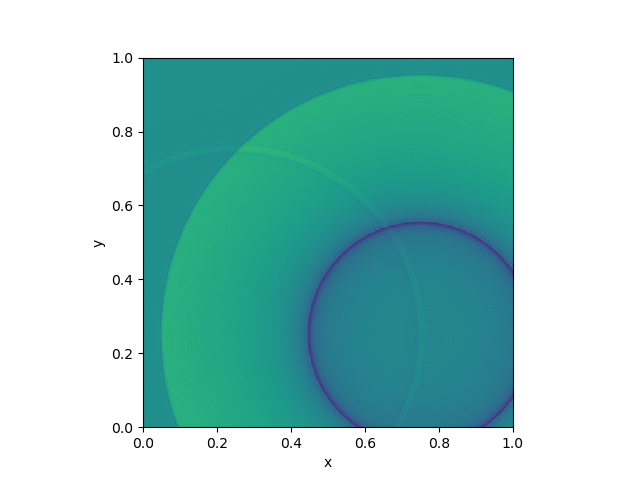
\includegraphics[width=\textwidth]{forward_perfect_matched_layer}
\end{figure}

\begin{figure}
    \caption{Решение прямой задачи с Perfect Matched Layer на границе - переменная скорость}
\noindent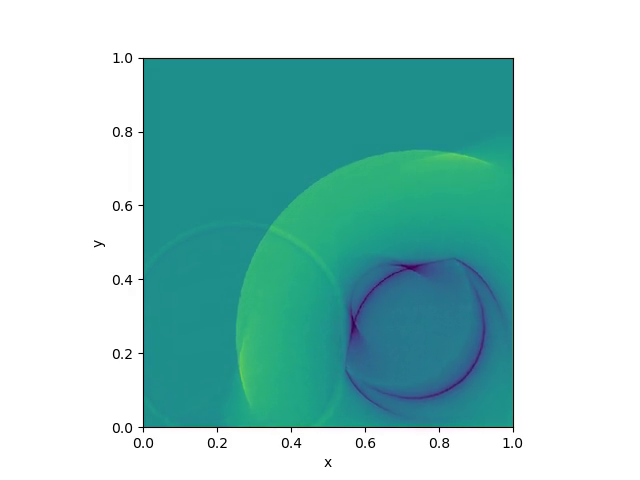
\includegraphics[width=\textwidth]{forward_perfect_matched_layer_variable_speed}
\end{figure}
